\documentclass[xcolor=dvipsnames]{beamer}


\usetheme[
          showdate=true,                     % show the date on the title page
          alternativetitlepage=true,         % Use the fancy title page.
          titlepagelogo=general_figures/shell,              % Logo for the fir\
st page.
          ]{UMD}

%\usetheme{Rochester}

%\usepackage{beamerthemesplit}
\usepackage{xmpmulti}

\usepackage{booktabs}
\usepackage{graphicx,float,wrapfig, bbm}
\usepackage{amsfonts, bbold, comment}
\usepackage{mdwlist}
\usepackage{tikz}
\usepackage{subfigure}
\usepackage{colortbl}

\usepackage{multirow}

\usetikzlibrary{shapes.geometric}
\definecolor{xred}{HTML}{DB4437}
\definecolor{xyellow}{HTML}{F4B400}
\definecolor{xgreen}{HTML}{0F9D58}

\newcommand*{\tcircle}[1]{\tikz[anchor=base,baseline=-2.5pt] \node[circle,fill=#1,scale=0.9] (X) {};}
\newcommand*{\tsquare}[1]{\tikz[anchor=base,baseline=-2.5pt] \node[fill=#1,scale=1.2] (X) {};}
\newcommand*{\tdiamond}[1]{\tikz[anchor=base,baseline=-2.5pt] \node[diamond,fill=#1,scale=0.7] (X) {};}
\newcommand*{\ttriangle}[1]{\tikz[anchor=base,baseline=-1.5pt] \node[regular polygon,regular polygon sides=3,fill=#1,scale=0.6] (X) {};}

\newcommand{\schedule}[0]{
\begin{frame}{Exhibition Schedule (Approximate)}

  \begin{itemize}
     \item[17:00] Presentation
     \item[17:20] Jeopardy! Champions vs. UMD Students' Systems
     \item[18:00] Q \& A
  \end{itemize}

  Find out more at {\bf qanta.org}.  We're looking for sponsors for
  prizes/events for human-computer question answering competitions at high school /
  college level.

\end{frame}
}


\newcommand{\fsi}[2]{
\begin{frame}[plain]
\vspace*{-1pt}
\makebox[\linewidth]{\includegraphics[width=\paperwidth]{#1}}
\begin{center}
#2
\end{center}
\end{frame}
}

\newcommand{\abr}[1]{\textsc{#1} }
\newcommand{\pos}[1]{{\texttt{#1}}}
\newcommand{\e}[2]{\mathbb{E}_{#1}\left[ #2 \right] }
\newcommand{\ind}[1]{\mathbb{I}\left[ #1 \right] }
\newcommand{\ex}[1]{\mbox{exp}\left\{ #1\right\} }
\newcommand{\g}{\, | \,}
\newcommand{\citename}[1]{#1 }

\newcommand{\gfxs}[2]{
\begin{center}
	\includegraphics[width=#2\linewidth]{simtrans/#1}
\end{center}
}

\newcommand{\gfxq}[2]{
\begin{center}
	\includegraphics[width=#2\linewidth]{qb/#1}
\end{center}
}



%\usecolortheme{ucdblack}
\title[HCQA]{Cooperative and Competitive Machine Learning through Question Answering}
\author{ Jordan Boyd-Graber et al.}
\date{2018}

\institute[Maryland] % (optional, but mostly needed)
{University of Maryland}

\begin{document}


\schedule{}

\frame{
\titlepage
\tiny
}

\fsi{qb/turing}{Turing Test: Definition of AI (Image from Wall Street
  International)}

\fsi{qb/jeopardy}{IBM Watson: QA Solved!}


\begin{frame}{But is Jeopardy! about Knowledge?}

  \begin{columns}
    \column{.25\linewidth}
    \gfxq{planet_money}{.75}
    \gfxq{jennings}{.7}    
    \gfxq{kenny_malone}{.7}
    \column{.7\linewidth}


    \small

    {\bf JENNINGS:} The deal with the buzzer is this. The buzzer is
    not live until Alex finishes reading the question. And if you buzz
    in before your buzzer goes live, \alert<1>{you actually lock yourself out
    for a fraction of a second}. So the big mistake on the show is
    people who are all adrenalized and are buzzing too quickly, too
    eagerly.

    \pause

    {\bf MALONE:} OK. To some degree, "Jeopardy!" is kind of a video game, and a \alert<2>{crappy video game where it's, like, light goes on, press button} - that's it.

    \pause
    
    {\bf JENNINGS:} (Laughter) Yeah.

    {\bf MALONE:} Is that true?

    {\bf JENNINGS:} I do like to think of it as a \alert<3>{beautiful art} and not a really crappy video game.
    
  \end{columns}
  

\end{frame}

\fsi{qb/jeopardy_qb}{}


\begin{frame}
	\frametitle{What is Quiz Bowl?}
	\begin{columns}

	\column{.5\linewidth}
	\begin{itemize}
		\item Two teams play each other
		\begin{itemize}
			\item Moderator reads a question
			\item When a team knows the answer, they signal (``buzz'' in)
			\item If right, they get points; otherwise, rest of the question is read to the other team
		\end{itemize}
		\item Hundreds of teams in the US alone
                \only<2>{\item Example \dots}
	\end{itemize}

	\column{.5\linewidth}
	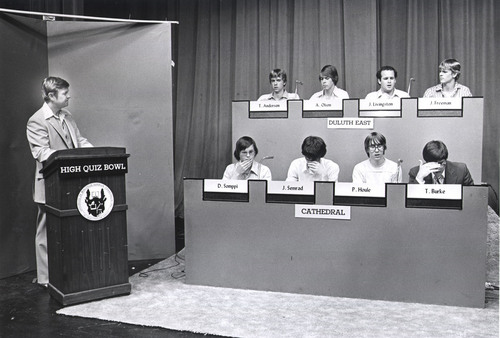
\includegraphics{qb/quizbowl}

	\end{columns}

\end{frame}

\begin{frame}[t]
	\frametitle{Sample Question}

        The Swiss-Italian architect Pietro Antonio Solari
        \only<2->{built several fortified towers in this city, which
          often vied for power with its northern rival Tver. A ruler
          of this city prevailed in the} \only<3->{Great Stand on the
          Ugra River. A prince from this city was nicknamed for
          winning a battle on the} \only<4->{Don river. Partly because
          a ruler of this city married} \only<5->{Sophia Palaiologina,
          the niece of the last Byzantine Emperor, this city styled
          itself the} \only<6->{``Third Rome'' after the fall of
          Constantinople. Another prince of this city stopped paying
          tribute to the} \only<7->{Mongols in 1476, ending the
          ``Tatar yoke.''} \only<8->{The Grand Duchy headquartered in
          this city came to an end in 1547 with the ascension of}
        \only<9->{ Ivan IV, who made it his capital. For 10 points,
          name this city where Ivan III renovated the
          Kremlin,} \only<10->{the capital of Russia.}\\
        \vspace{.5cm} \only<11->{ {\bf Moscow} (Moskva / Muscovy)}

\end{frame}


\begin{frame}
	\frametitle{Question Structure Enables Compeition}

	\begin{columns}
		\column{.5\linewidth}

		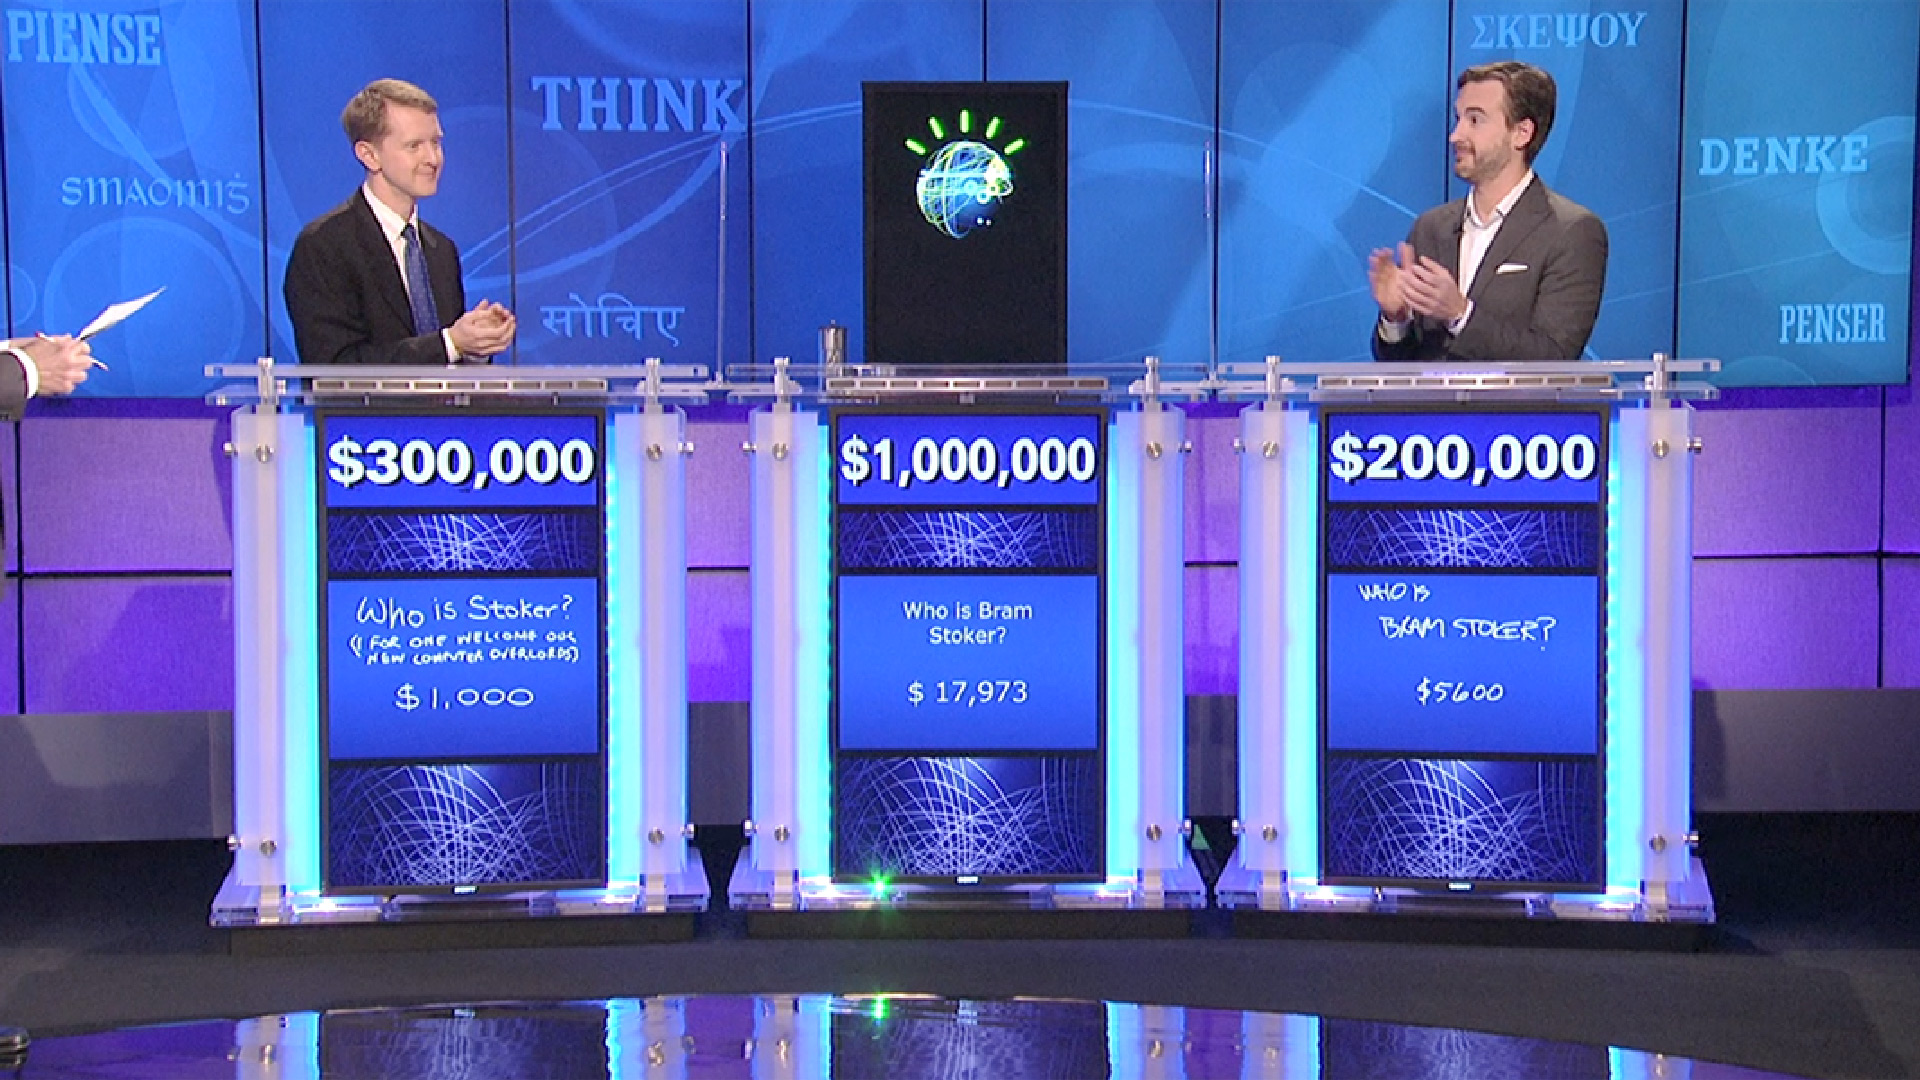
\includegraphics[width=1.0\linewidth]{qb/jeopardy}


		\column{.5\linewidth}
		\begin{itemize}
                        \item Watson must decide to answer {\bf once}, after
                          complete question
                        \item Quiz Bowl: decide after each word
                        \item Obscure clues at start, easy at end
                        \item ``Gold standard'' in trivia community
		\end{itemize}

	\end{columns}

\end{frame}


\begin{frame}{How to approach this problem \dots}

    \only<1>{
  \begin{columns}
    \column{.5\linewidth}
    \gfxq{guess}{0.8}
    \column{.5\linewidth}
    \gfxq{buzzer}{0.8}
  \end{columns}
}
\only<2>{
   \gfxq{guess}{0.5}
}
\end{frame}


\begin{frame}{Homework 1--2: Vector Space Model}

  \only<1>{\gfxq{unigram_models_0}{.8}}
  \only<2>{\gfxq{unigram_models_1}{.8}}
  \only<3>{\gfxq{unigram_models_2}{.8}}
  \only<4>{\gfxq{unigram_models_3}{.8}}
  \only<5>{\gfxq{unigram_models_4}{.8}}
  \only<6>{\gfxq{unigram_models_5}{.8}}
  \only<7>{\gfxq{unigram_models_6}{.8}}
  \only<8>{\gfxq{unigram_models_7}{.8}}
  \only<9>{\gfxq{unigram_models_8}{.8}}


\end{frame}


% \begin{frame}{Training}

%   \begin{columns}
%     \column{.5\linewidth}
%       \begin{itemize}
%         \item Initialize embeddings from \textsc{word2vec}
%         \item Randomly initialize composition matrices
%         \item Update using \textsc{warp}
%           \begin{itemize}
%             \item Randomly choose an instance
%             \only<2->{\item Look where it lands}
%             \only<4->{\item Has a correct answer}
%             \only<5->{\item Wrong answers may be closer}
%             \only<6->{\item Push away wrong answers
%             \item Bring correct answers closer}
%           \end{itemize}
%       \end{itemize}

%     \column{.5\linewidth}

%       \only<1>{\gfxq{warp_training_5}{.8}}
%       \only<2>{\gfxq{warp_training_4}{.8}}
%       \only<3>{\gfxq{warp_training_3}{.8}}
%       \only<4>{\gfxq{warp_training_2}{.8}}
%       \only<5>{\gfxq{warp_training_1}{.8}}
%       \only<6>{\gfxq{warp_training_0}{.8}}
%   \end{columns}

% \end{frame}


\begin{frame}{Homework 4: More complicated representations}

  \gfxq{embedding}{1.0}

\end{frame}


\begin{frame}{How to approach this problem \dots}

    \only<1>{
  \begin{columns}
    \column{.5\linewidth}
    \gfxq{guess}{0.8}
    \column{.5\linewidth}
    \gfxq{buzzer}{0.8}
  \end{columns}
}
\only<2>{
   \gfxq{buzzer}{0.5}
}
\end{frame}



\begin{frame}
\frametitle{How to know if you're doing well?}

\begin{columns}

	\column{0.5\linewidth}

	\begin{center}
		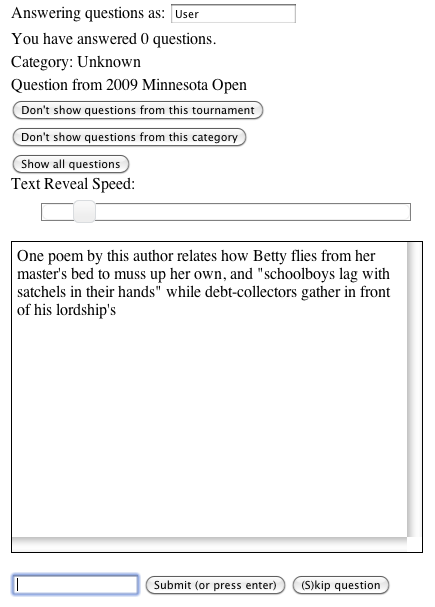
\includegraphics[width=0.8\linewidth]{qb/screenshot}
	\end{center}

	\column{0.5\linewidth}


	\only<2>{
	\begin{itemize}
		\item 7000 questions: first day
		\item 43000 questions: two weeks
		\item 461 unique users
                \item Imitated \dots
	\end{itemize}
        \gfxq{protobowl}{.8}
	}



\end{columns}
\end{frame}

\begin{frame}{Homework 5: Learning to to Buzz}

  \gfxq{player_profile}{.9}

  \pause
  Varies by category!

\end{frame}


\begin{frame}{But First\dots Not all Fun and Games: Simultaneous Interpretation}

  \begin{columns}
    \column{.5\linewidth}
  \begin{itemize}
    \item Exhausting for humans
    \item Computers not trusted
    \item Differential strengths
    \item Same word-by-word characteristic
  \end{itemize}

  \column{.5\linewidth}
 \gfxs{computer-interpreter}{1.0}
 \end{columns}
\end{frame}

\begin{frame}{Today's Match}

  \begin{block}{Computers}
    \begin{itemize}
    \item Fall 2018: CMSC 723 (Forward Rethinking)
    \item Spring 2019: CMSC 470 (QANTA
      Handle Us)
    \end{itemize}
  \end{block}

  \begin{block}{Humans}
    \gfxq{2019_may_expo}{.8}
  \end{block}

  Forty questions artisinally selected from Maryland's 2019 Terrapin
  Invitational Tournament's first four packets
  
\end{frame}

\schedule{}

% \begin{frame}{Exhibition Match!}

%   \begin{columns}
%     \column{.5\linewidth}
%     \gfxq{joker}{.8}
%     \gfxq{final_jeopardy}{.8}
%     \column{.5\linewidth}
%     \gfxq{maqt}{.8}
%     \gfxq{maqt_naqt_d2}{.8}
%   \end{columns}

% \end{frame}

\schedule{}


% Hard but not really a good question: F3 Q24

\begin{frame}{Impossible Until the End}
\alert<3>{Ritchie Watson commended this play's historical accuracy for
  getting the price for a dozen eggs right---ten cents---to defend
  against Elizabeth Hardwick’s contention that it was a sentimental
  history.} \alert<4>{At the end of this play, a man wonders why a wheelchair is
at the top of a staircase, and} \alert<5>{Alexandra announces that she is leaving
her mother. Leo is pressured into stealing a set of valuable railroad
bonds in this drama. In this play, which takes its title from the Song
of Solomon,} Regina Hubbard schemes  \tdiamond{xgreen}
\tcircle{xgreen} to obtain a majority share in a cotton mill. For 10
points,  \tsquare{xgreen}  \ttriangle{xgreen} name this play by
Lillian Hellman. \\

\pause

\textbf{Answer}: The\ Little\ Foxes\\

\only<3>{Academic literature}
\only<4>{Vague plot summary}
\only<5>{Avoid last names}

\end{frame}

% Tricky and hard: F3 Question 25

\begin{frame}{Tricky and impossible for current systems}
In Our Town, a character  \ttriangle{xred} with this given name explains Grover’s Corners’ place in the universe. In The Crucible, a character  \tcircle{xred} with this first name contends that the girls’ actions are part of their “silly seasons” and is the wife of Francis Nurse. A novel with this name, which conducts hidden messages to Rommel in The English Patient, is titled for a character who is killed in a boating accident at Manderley. For 10 points, give this name of a Daphne du Maurier  \tdiamond{xyellow}  \tsquare{xgreen} gothic novel which is also the first name of Miss Sharp, the protagonist of William Thackeray's Vanity Fair. \tcircle{gray}  \ttriangle{gray}


\ttriangle{xred} Thornton Wilder
\tcircle{xred} Richard
\tcircle{gray} Richard
\ttriangle{gray} Thornton Wilder \\
\textbf{Answer}: Rebecca\\
\end{frame}

% Tricky and hard: F3 Question 29

\begin{frame}{Close, but \dots}
An army that took its name from this geographical feature had a
British doctor, James Paroissien, as its Surgeon General, and recent
scholarship by Peter Blanchard revealed its use of slaves. That army
crossed this geographical feature according  \ttriangle{xred} to
Thomas Maitland’s  \tcircle{xred} plans at Uspallata and Los
Patos. Spanish forces under Rafael Maroto were defeated in the
foothills of these mountains by an army led by José de San Martín and
Bernardo O'Higgins.  \tsquare{xred} For 10 points, name this mountain
range of South America that played a role  \ttriangle{xyellow} in the
independence of Chile. \tdiamond{gray}  \tcircle{gray}  \tsquare{gray}

\ttriangle{xred} Angel Falls
\tcircle{xred} Mountain
\tsquare{xred} Battle of Chacabuco
\tdiamond{gray} Battle of Chacabuco
\tcircle{gray} Mountain
\tsquare{gray} Battle of Chacabuco \\
\pause
\textbf{Answer}: Andes\\

\end{frame}

% Showing strength of QB format: Packet F3 Question 30

\begin{frame}{Showing the strength of quiz bowl format}
A painting by this artist  \tsquare{xred} presents a tree as a cupboard with two doors, behind which are a white sphere and a miniature lighted house. A series of three paintings by this man shows a daytime sky with cumulus clouds above a dark house illuminated by a lamppost. This artist of Blood Will Tell and The Empire of Lights depicted a clock set to 12:43  \tcircle{xgreen} as a locomotive speeds out of a fireplace and a man in  \tsquare{xyellow} a bowler hat with an  \ttriangle{xgreen} apple in front of his face. For 10 points, name this Belgian surrealist painter  \tdiamond{xgreen} of the Son of Man and Time Transfixed.

\tsquare{xred} Argon \\
\pause
\textbf{Answer}: René\ Magritte\\
\end{frame}

% Why it's a good learning framework: Packet F3 Question 31


\begin{frame}{Our QA Systems are Crazy}

\only<1-2>{
\begin{block}{Out of Touch}
On "The Critic", this man was replaced by a drunken animatronic bear from the Country Bear Jamboree but nobody seemed to notice.  This man was edited to appear in the film "Contact", which prompted an angry statement from Mike McCurry.  He was portrayed by Dennis Quaid in "The Special Relationship", who ate McDonald's every day to prepare for the role.  A fictionalized version of this man named Henry Burton, a charismatic Southern governor running for the Democratic nomination, is portrayed by John Travolta in "Primary Colors".  For ten points, name this American president who played the saxophone on an appearance on the Arsenio Hall Show.
\end{block} }
\only<2>{{\bf Samuel L. Jackson?}}

\end{frame}


\begin{frame}{Matching Entites Across Sentences}

\begin{block}{\only<2->{Magic Flute}}

    At its premiere, \alert<3>{the librettist of this opera} portrayed
    \alert<4>{a character who asks for a glass of wine with his dying wish}. \alert<4>{That
    character} in this opera is instructed to ring some bells to summon
    his love. At its beginning, \alert<5>{a man} who claims to have killed a (*)
    serpent has a padlock put on \alert<5>{his} mouth because of \alert<5>{his} lying. The
    plot of this opera concerns a series of tests that \alert<5>{Tamino} must
    undergo to rescue Tamina from Sorastro. For 10 points, name this
    Wolfgang Mozart opera titled for \alert<6>{an enchanted woodwind instrument}.
\end{block}



\only<3-4>{{\bf Not all references are named (\alert<3>{Emanuel
      Schikaneder}, \alert<4>{Papageno})}}
\only<5>{Need to be able to match pronouns across sentences (or have
  deep world knowledge)}
\only<6>{Requires semantic knowledge}
\end{frame}



\begin{frame}{}

  \begin{columns}
    \column{.4\linewidth}
        
\includegraphics[width=0.8\linewidth]{general_figures/hehe} \\
        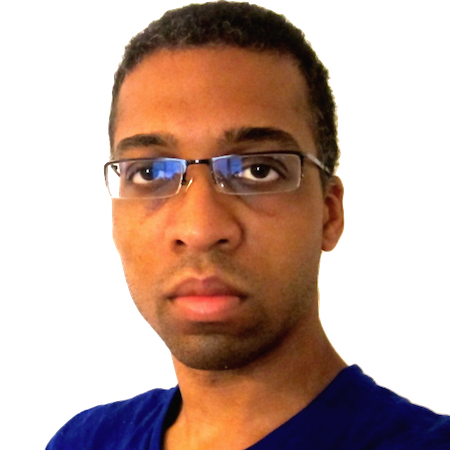
\includegraphics[width=0.8\linewidth]{general_figures/alvin}
    \column{.6\linewidth}

        \begin{block}{ {\bf \href{http://umiacs.umd.edu/~jbg//docs/2015_emnlp_rewrite.pdf}{Syntax-based Rewriting for Simultaneous Machine Translation}}}
He He, Alvin Grissom II, {\bf Jordan Boyd-Graber}, and Hal {Daum\'{e} III}.  \emph{Empirical Methods in Natural Language Processing}, 2015
        \end{block}

        \begin{block}{ {\bf \href{http://umiacs.umd.edu/~jbg/docs/2016_naacl_interpretese.pdf}{Interpretese vs. Translationese: The Uniqueness of Human Strategies in Simultaneous Interpretation}}}
He He, {\bf Jordan Boyd-Graber}, and Hal {Daum\'{e} III}.
\emph{North American Association for Computational Linguistics}, 2016
        \end{block}

  \end{columns}


\end{frame}


\begin{frame}{Human-Computer Question Answering}

  \begin{itemize}
    \item Pit machine learning algorithms against humans
    \item Fun task for human participants
    \item Good system for discriminating depth and confidence of
      algorithms
    \item Knowledge and language comprehension needed to do well
    \item Simple approaches work well if you have the whole question
    \item Good competition for QA systems
    \item Can get much harder
      \begin{itemize}
        \item Speech
       \item Specialized knowledge
        \item Adversarial authoring
      \end{itemize}
  \end{itemize}

\end{frame}


\begin{frame}{Future \dots}

  \begin{itemize}
    \item Computers dominate on ``normal'' questions
    \item Not so much on adversarial questions
    \item Stronger QA systems (e.g., Google's!)
      \begin{itemize}
        \item Need more thought on how to explain
        \item Expose QA system to more users
        \item Increase the breadth of resources
        \item Multilingual
      \end{itemize}
  \end{itemize}

\end{frame}





\begin{frame}{Find out More!}

		\begin{itemize}
			\item Code: \url{http://github.com/Pinafore/qb}
                        \item Shared Task \url{http://qanta.org}
		\end{itemize}

\end{frame}

\fsi{qb/trick/round_one}{Round 1: Only IR-based QA system}
\fsi{qb/trick/round_two}{Round 2: RNN-based QA system}


% \begin{frame}{Come to UMD}

% \begin{columns}
% 	\column{.5\linewidth}
%         \only<1>{
%         	\begin{center}
% 		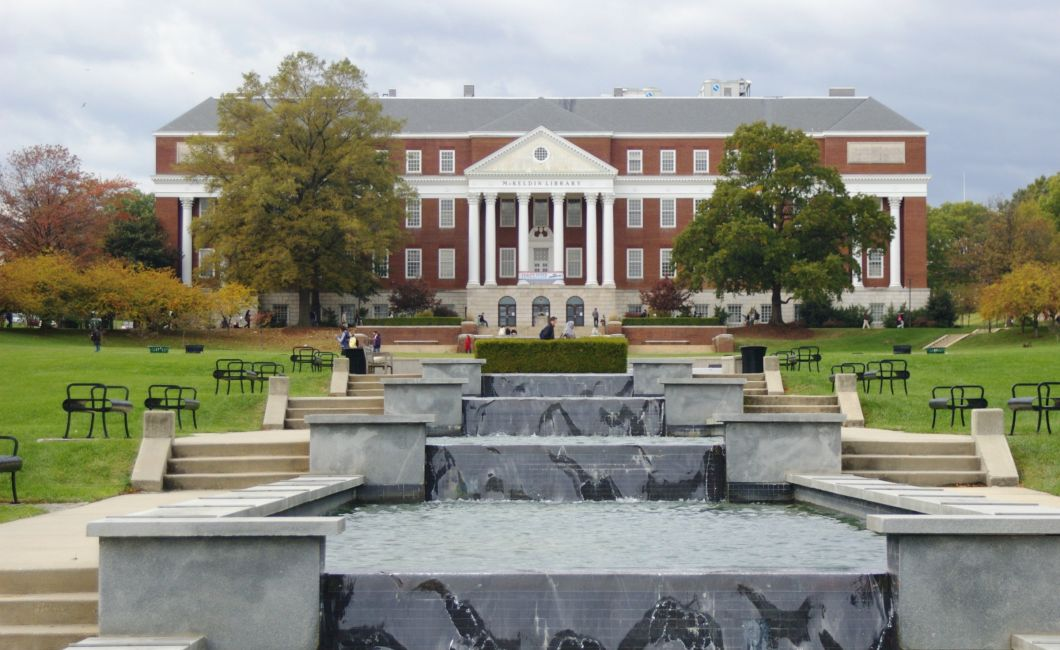
\includegraphics[width=.9\linewidth]{umd/umd} \\
% 		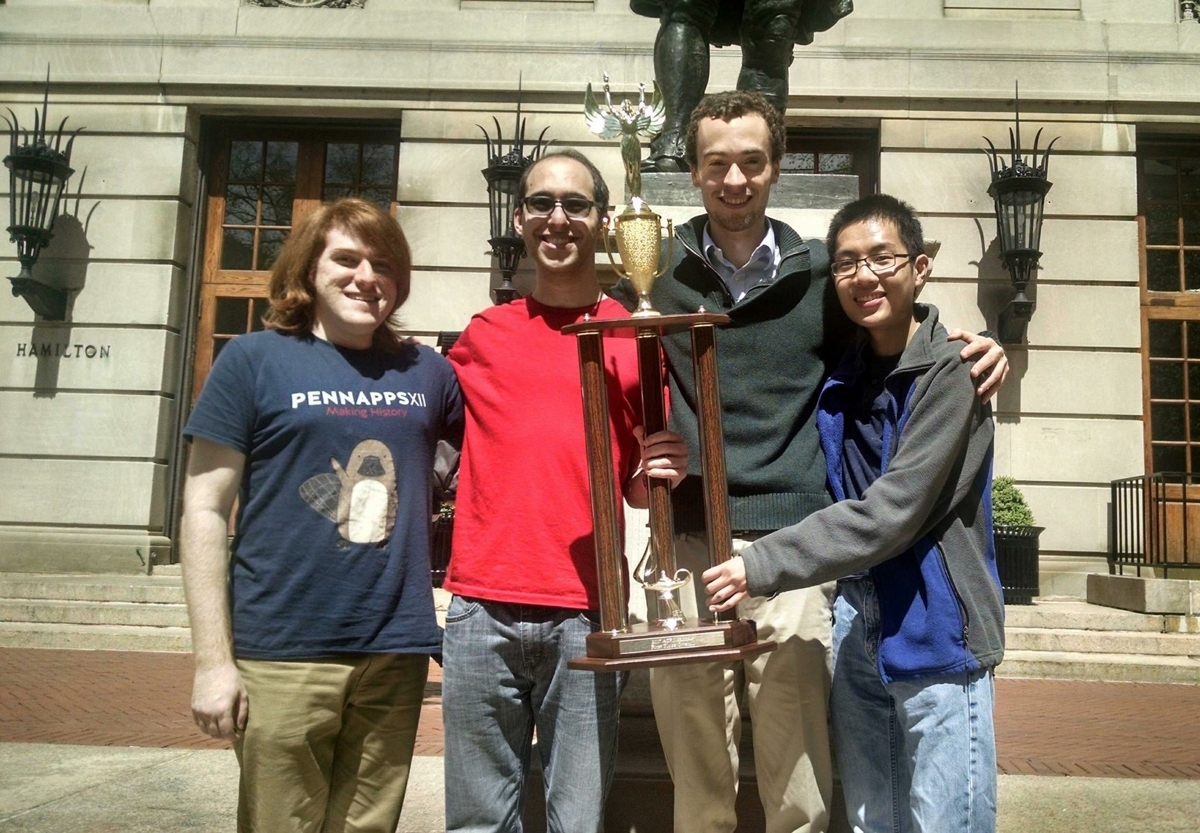
\includegraphics[width=.9\linewidth]{umd/qb_team}
% 	\end{center}
%               }
% 	\column{.5\linewidth}
% 		\begin{itemize}
%                 \item Looking for undergrads/grads/interns
%                 \item A great place for natural language
%                   processing and machine learning
%                 \item Not too shabby at quiz bowl either
% 		\end{itemize}
% \end{columns}

% \end{frame}

\frame{
  \frametitle{But wait, there's more!}

  \vspace{-.5cm}

\begin{columns}



  \column{.5\linewidth}

   \begin{block}{Computational Social Science}
     \centering
     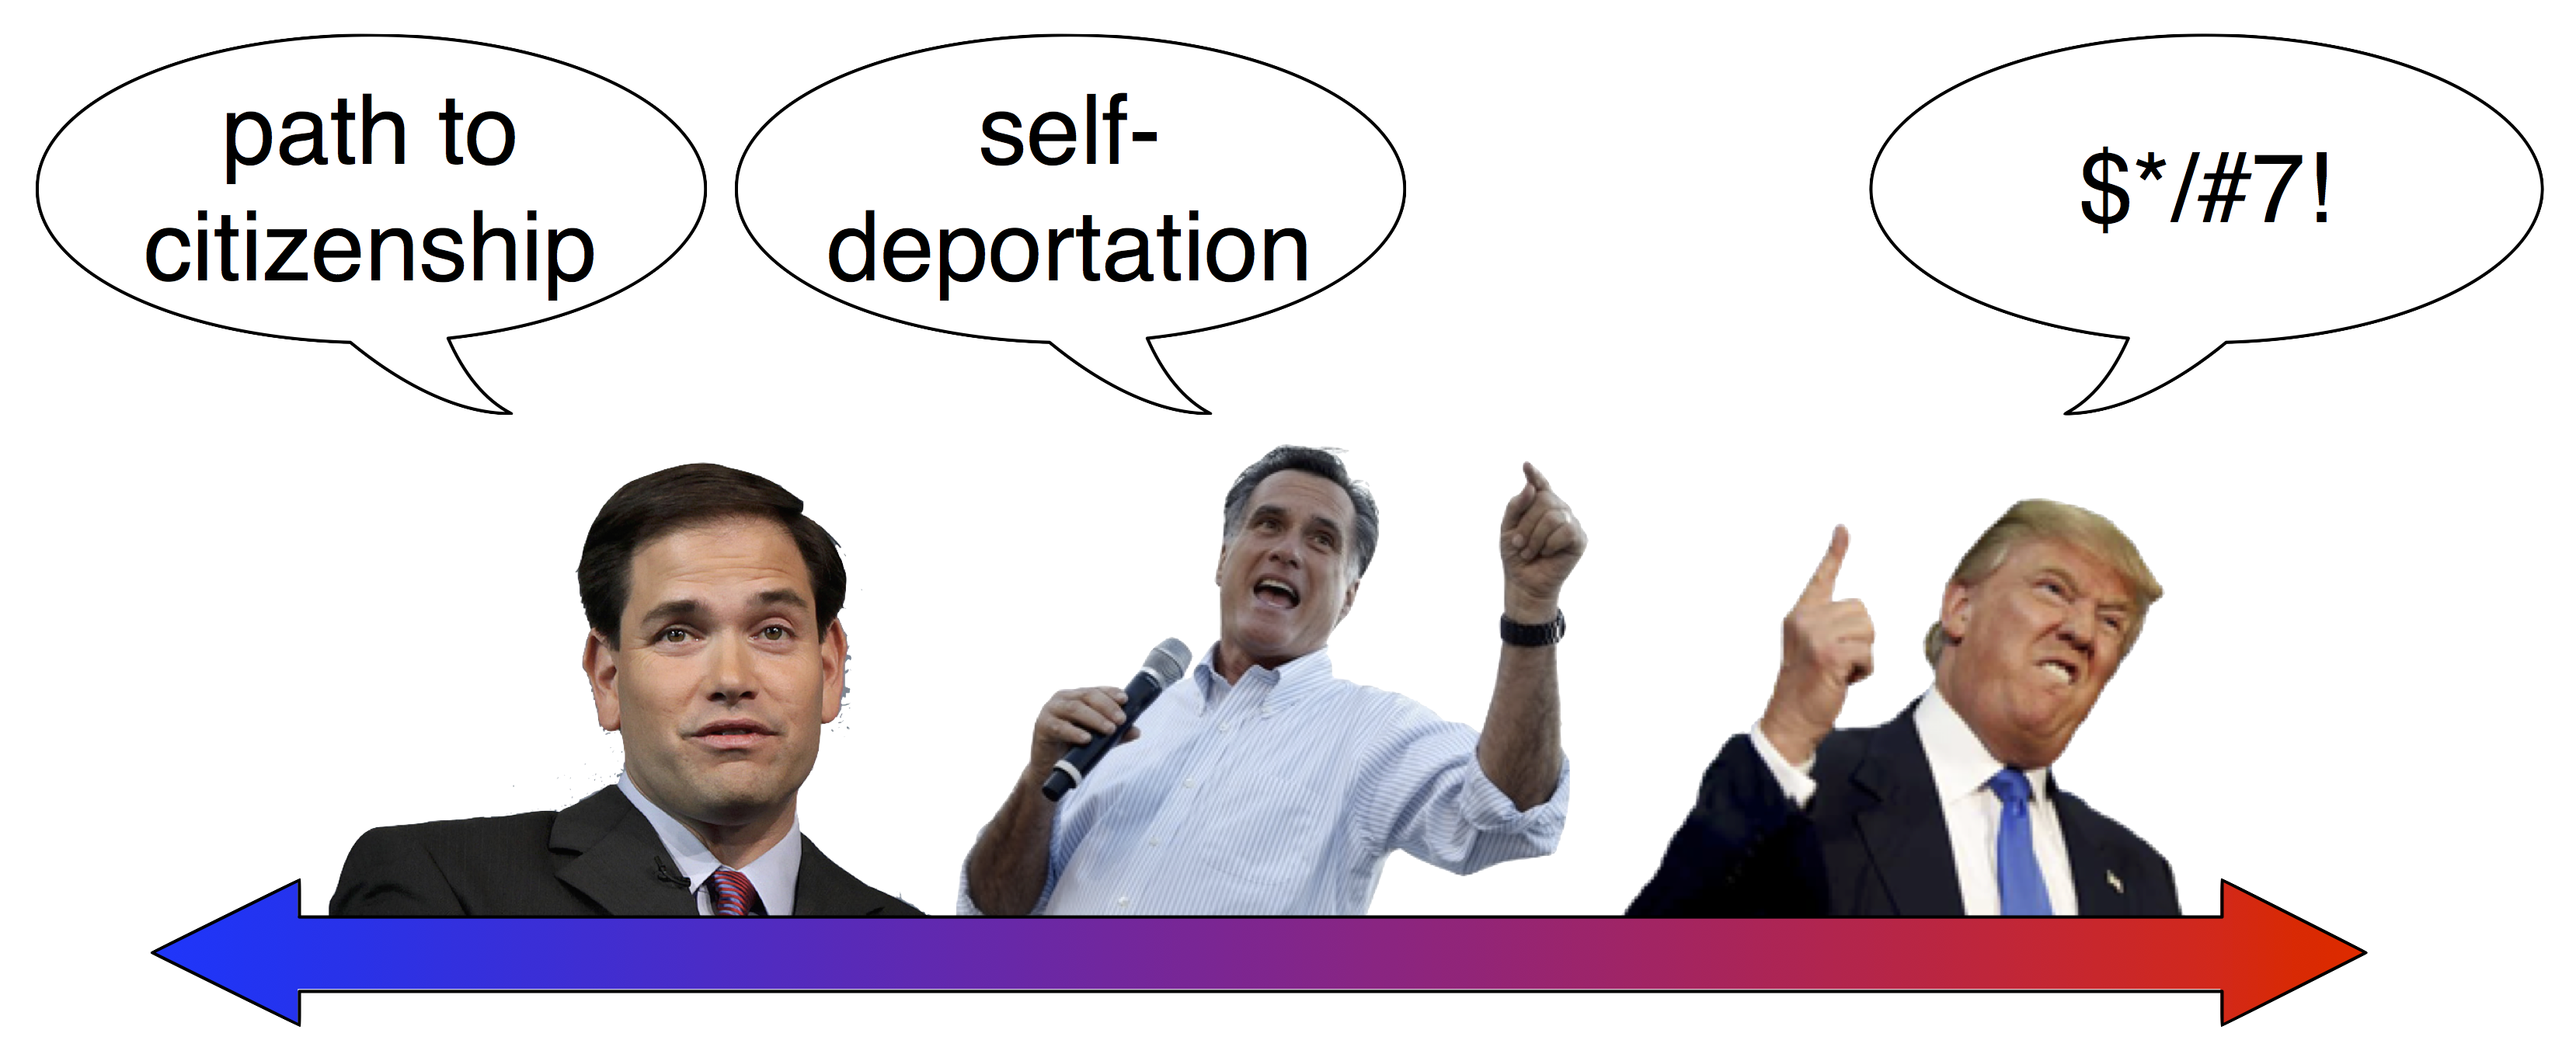
\includegraphics[width=0.9\linewidth]{teaparty/figures/framing} \\
     \cite{nguyen-13b,nguyen-15}
   \end{block}


    \begin{block}{Interactive Machine Learning}
     \centering
        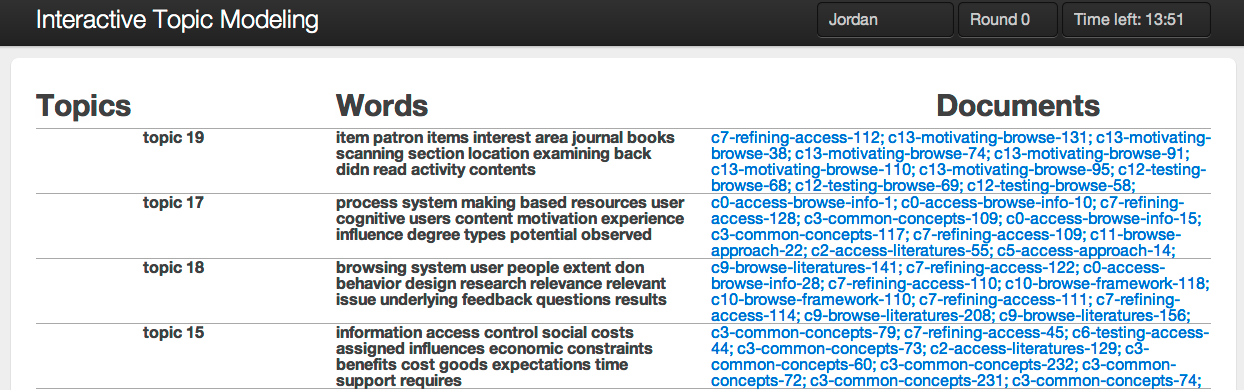
\includegraphics[width=0.4\linewidth]{interactive_topic_models/new_interface} \\
       \cite{Smith-17,Poursabzi-16}
    \end{block}


  \column{.5\linewidth}


    \begin{block}{Multilingual Topic Models}
      \begin{center}
        \begin{large}
          $p_{\mbox{topic}}(e | f)$ \\
         \end{large}
      \cite{eidelman-12,hu-14}
       \end{center}
    \vspace{-.3cm}
    \end{block}


    \begin{block}{Sentiment / Internal State}
    \centering
        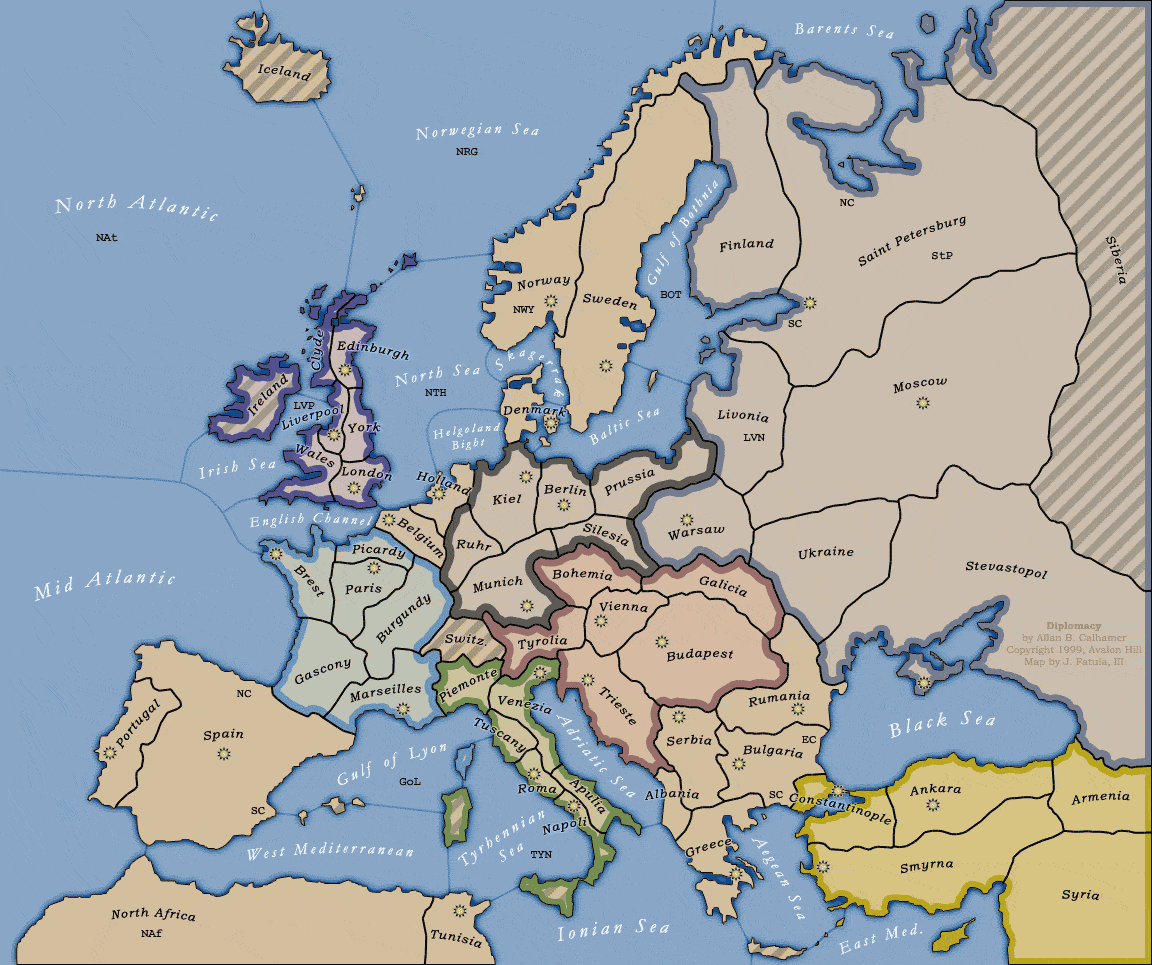
\includegraphics[width=0.4\linewidth]{general_figures/diplomacy} \\
        \cite{niculae-15,sayeed-12,boyd-graber-10}
    \end{block}




\end{columns}

}




\frame{

	\frametitle{Thanks}

        \begin{block}{Collaborators (not listed on previous slides)}
          Anupam Guha (Maryland), Manjhunath Ravi (Colorado), Danny Bouman (UMD UG),
          Stephanie Hwa (UMD UG), Yogarshi Vyas (UMD), Larry Davis
          (UMD), Naho Orita (Tohoku), Snigdha Chaturvedi (UMD), Varun
          Manjunatha (UMD), Srijan Kumar (UMD), Vlad Niculae
          (Cornell), Cristian Danescu-Niculescu-Mizil (Cornell),
          Richard Socher (Salesforce), Leonardo Claudino (UMD)
        \end{block}

	\begin{columns}

	\column{.5\linewidth}
        \begin{block}{Funders}
        \begin{center}
          
\includegraphics[width=0.4\linewidth]{general_figures/nsf}
       \end{center}
        \end{block}

	\column{.5\linewidth}
        \begin{block}{Supporters}
        	\gfxq{naqt}{.4}
        \end{block}

        \end{columns}
}

\begin{frame}[plain]

\begin{columns}
  \column{.3\linewidth}
        \begin{center}
          @boydgraber
          
\includegraphics[width=0.6\linewidth]{general_figures/twitter}
          \\
          \end{center}
  \column{.65\linewidth}

  \begin{center}
    https://www.youtube.com/c/JordanBoydGraber
    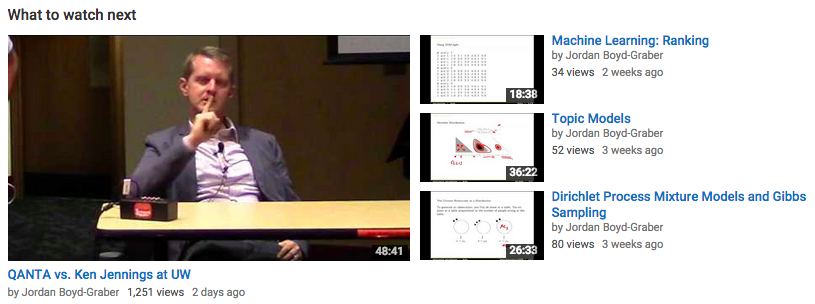
\includegraphics[width=1.0\linewidth]{general_figures/youtube} \\

\end{center}

\end{columns}

\begin{center}
\huge
http://qanta.org \\
http://boydgraber.org
       \end{center}


\end{frame}

\begin{frame}{References}
\bibliographystyle{style/acl}
\tiny
\bibliography{bib/journal-full,bib/jbg}
\end{frame}




\begin{frame}{How can this fail?}

  \only<1>{\gfxq{opponent_fail1}{.8}}
  \only<2>{\gfxq{opponent_fail2}{.8}}
  \only<3>{\gfxq{opponent_fail3}{.8}}
  \only<4>{\gfxq{opponent_fail4}{.8}}
  \only<5>{\gfxq{opponent_fail5}{.8}}
  \only<6>{\gfxq{opponent_fail6}{.8}}
  \only<7>{\gfxq{opponent_fail7}{.8}}

\end{frame}

\begin{frame}{Can we do better?}

  \only<1>{\gfxq{dqn_overview2}{.8}}
  \only<2>{\gfxq{dqn_overview3}{.8}}
  \only<3>{\gfxq{dqn_overview4}{.8}}

\end{frame}


\begin{frame}{Comparing Models}

  \begin{itemize}
    \item Single-Player
    \item Deep Q-Network (DQN): World=Opponent~\cite{mnih-15}
      \begin{itemize}
        \item Learn representation of state to estimate $Q$-function
        \item Generalization of regression-based methods
        \item Similar to our representation of content
      \end{itemize}
    \item Deep Reinforcement Opponent Network (DRON)
  \end{itemize}

\end{frame}


\begin{frame}[plain]


\only<4->{\vspace{-.5cm}}

  \begin{columns}[T]
    \column{.3\linewidth}

    \only<1->{ 
\includegraphics[width=2\linewidth]{qb/feature_ex_l_1} \\ }
    \vspace{.5cm}
    \only<4->{ 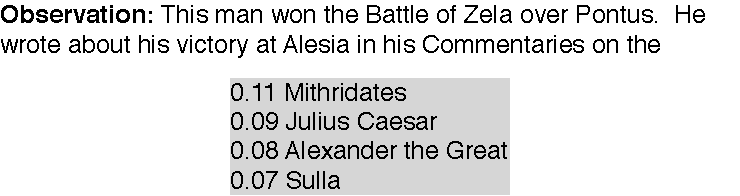
\includegraphics[width=2\linewidth]{qb/feature_ex_l_2}  \\ }
    \vspace{.5cm}
    \only<7->{ 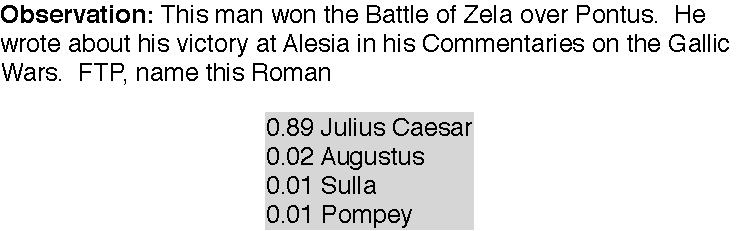
\includegraphics[width=2\linewidth]{qb/feature_ex_l_3}  \\ }


    \column{.68\linewidth}
    \vspace{-.5cm}
    \only<2->{ 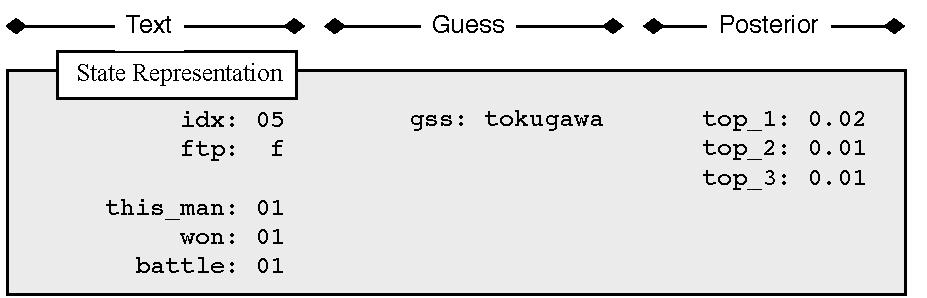
\includegraphics[width=.85\linewidth]{qb/feature_ex_r_1} \\ }
    \only<3->{ \vspace{-.5cm} \hspace{.5cm} 
\includegraphics[width=.1\linewidth]{qb/feature_ex_wait}  \\ }
    \only<5->{ 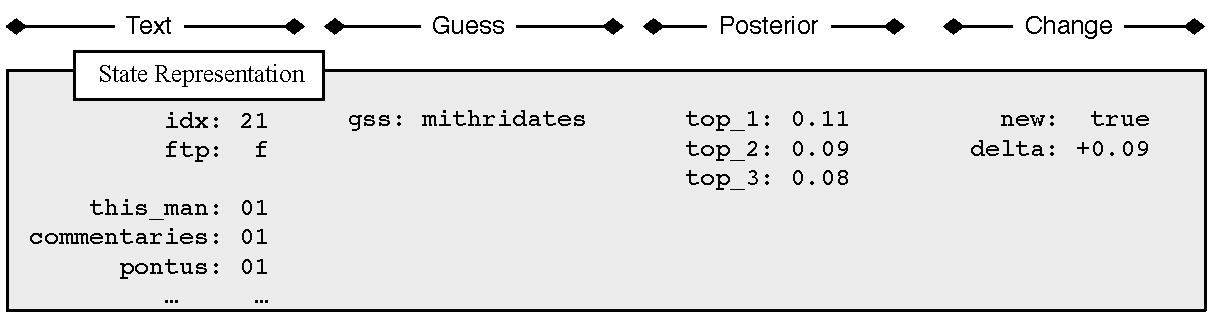
\includegraphics[width=\linewidth]{qb/feature_ex_r_2} \\ }
    \only<6->{ \vspace{-.5cm} \hspace{.5cm}
\includegraphics[width=.1\linewidth]{qb/feature_ex_wait}  \\ }
    \only<8->{ 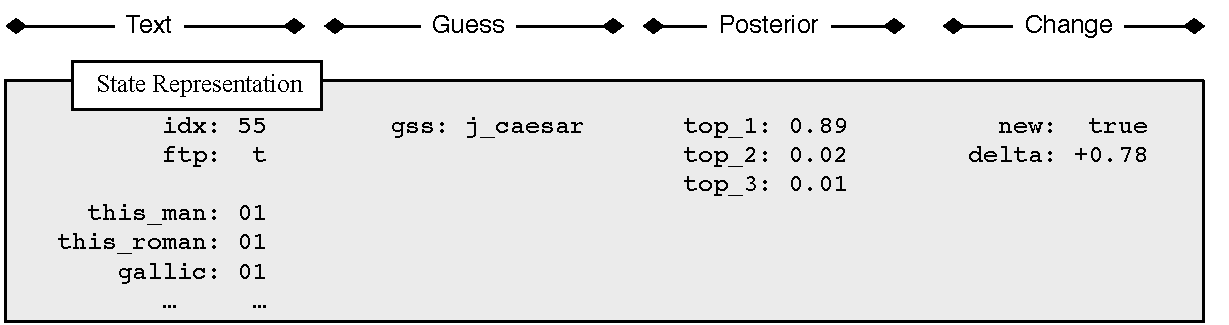
\includegraphics[width=\linewidth]{qb/feature_ex_r_3} \\ }
    \only<9->{ \vspace{-.5cm} \hspace{.5cm} 
\includegraphics[width=.1\linewidth]{qb/feature_ex_buzz}  \\ }
    \only<9->{Answer: {\bf Julius Caesar}}
  \end{columns}

\end{frame}


\begin{frame}{Add more features: DRON-concat}

  \gfxq{dron-concat}{.8}

\end{frame}


\begin{frame}{Error Analysis}

  \only<1>{\gfxq{error1}{.8}}
  \only<2>{\gfxq{error2}{.8}}
  \only<3>{\gfxq{error3}{.8}}
  \only<4>{\gfxq{error4}{.8}}
  \only<5>{\gfxq{error5}{.8}}
  \only<6>{\gfxq{error6}{.8}}
  \only<7>{\gfxq{error7}{.8}}

\end{frame}



\begin{frame}{How the shared task works}

\begin{columns}
  \column{.3\linewidth}
  \gfxq{bamber}{.5}

  \column{.65\linewidth}
  \begin{itemize}
    \item<3-> Hi! Available questions are \texttt{[1,2,3,4]}
    \item<5-> It's \texttt{Extremism}
    \item<7-> It's \texttt{in}
    \item<9-> It's \texttt{the}
    \item<11-> Got it!  You've answered Question 1 at Position
      3 with \texttt{Barry\_Goldwater}
  \end{itemize}

\end{columns}


\begin{columns}

  \column{.65\linewidth}
  \begin{itemize}
    \item<2-> I'm User~1.  I’d like to play!
    \item<4-> I’d like to hear Word~1 of Question 1
    \item<6-> I’d like to hear Word~2 of Question 1
    \item<8-> I’d like to hear Word~3 of Question 1
    \item<10-> I’d like to answer Question 1 with
      \texttt{Barry\_Goldwater}
    \end{itemize}
  \column{.3\linewidth}
  \only<2->{\gfxq{buzzer}{.5}}
\end{columns}

\end{frame}


\begin{frame}{Are there enough opportunities?}


\begin{center}
\begin{tabular}{lcccc}
\toprule
& \alert<2>{verb} & \alert<3>{voice} & \alert<4>{noun} & \alert<5>{clauses} \\
\midrule
Applicable \% & \only<2->{39.9} & \only<3->{50.0} & \only<4->{26.4} & \only<5->{4.8} \\
Accepted \% & \only<2->{22.5} & \only<3->{24.0} & \only<4->{51.2} & \only<5->{38.4} \\
\bottomrule
\end{tabular}
\end{center}

\only<2>{
\begin{itemize*}
\item[O:] {\bf They announced} that the president will restructure the division.
\item[R:] The president will restructure the division, {\bf they announced}.
\end{itemize*}
}


\only<3>{
  \begin{columns}
    \column{.4\linewidth}

    \gfxs{rewrite_input}{.9}
    \column{.55\linewidth}
    \vspace{-.5cm}
    \gfxs{rewrite_transform}{.9}
   \end{columns}
}

\only<4>{
\begin{itemize*}
  \item[O:] the e-mail server of Clinton
  \item[R:] Clinton's e-mail server
\end{itemize*}
}

\only<5>{
\begin{itemize*}
\item[O:] \pos{S}$_1$ \pos{conj} \pos{S}$_2$: We should march {\bf because} winter is coming.
\item[O:] \pos{conj} \pos{S}$_2$, \pos{S}$_1$: {\bf Because} winter is
  coming, we should march.
\vspace{1cm}
\item[R:] \pos{S}$_2$, \pos{conj'} \pos{S}$_1$: Winter is coming, {\bf because of this}, we should march.
\end{itemize*}
}


\end{frame}

\begin{frame}{}

\gfxs{rewrite_eval}{.8}
\pause
We rewrite 32.2\% of
sentences, reducing the delay from 9.9 words/seg to 6.3 words/seg per
segment for rewritten sentences and from 7.8 words/seg to 6.7 words/seg overall.

\end{frame}

\begin{frame}{How good are the translations?}

  \gfxs{tradeoff-rw-bleu}{.7}

\begin{center}
Aggressiveness based on different right probability thresholds
\cite{fujita-13}
\end{center}

\end{frame}

\begin{frame}{Why does the quality improve?}

\begin{center}
\begin{tabular}{ccccc}
\toprule
& \multicolumn{3}{c}{Translation} & \\
\cmidrule{2-4}
& \abr{gd} & \abr{rw} & \abr{rw+gd} & Gold ref \\
\midrule
\# of verbs & 1971 & 2050 & {\bf 2224} & 2731 \\
\bottomrule
\end{tabular}
\end{center}

\end{frame}

\begin{frame}{Future Steps}

  \begin{itemize}
    \item Verb prediction through argument structure \only<2->{(entity
        / coref)}
    \item Richer translation model~\cite{oda-15,cho-16}
    \item Better reward (e.g., MEANT)  \only<3->{(richer answer space)}
    \item Paraphrase database
    \item Learning from imperfect feedback  \only<4->{(player clues)}
    \item Centaur translations  \only<5->{(centaur QB)}
  \end{itemize}

\end{frame}

\begin{frame}{Where we have problems}

\only<1-2>{
\begin{block}{Out of Date}
Although he won the California primary in 2000, he distanced himself
from fellow reform presidential candidate Pat Buchanan by comparing
him to Attila the Hun. After being called a jackass, he prompted
Lindsey Graham to destroy his phone by giving out his number during a
speech. The slogan (*) Make America Great Again has been used by this
politician, who claimed he didn't like people who were captured as a
slight to John McCain and kicked off his 2016 presidential bid with
some inflammatory remarks about Mexicans. For 10 points, name this
Republican candidate and real estate mogul.
\end{block} }
\only<2>{{\bf Chris Christie?}}

\only<3-4>{
\begin{block}{Out of Touch}
  This singer recently cancelled the Great Escape Tour, and, in one
  song, she claims that she will be ``Eating crumpets with the sailors
  / On acres without the neighbors.'' She collaborated with Jennifer
  (*) Hudson on the song ``Trouble,'' which was issued in her album
  update Reclassified. This artist of ``Change Your Life'' was
  inspired by scenes from the movie Clueless to make the music video
  for a song in which she collaborated with Charli XCX. For 10 points,
  name this Australian rapper whose album The New Classic contained
  ``Fancy.''
\end{block} }
\only<4>{{\bf Bruce Springsteen?}}

\end{frame}



\end{document}
